\documentclass[]{article}
\usepackage{lmodern}
\usepackage{amssymb,amsmath}
\usepackage{ifxetex,ifluatex}
\usepackage{fixltx2e} % provides \textsubscript
\ifnum 0\ifxetex 1\fi\ifluatex 1\fi=0 % if pdftex
  \usepackage[T1]{fontenc}
  \usepackage[utf8]{inputenc}
\else % if luatex or xelatex
  \ifxetex
    \usepackage{mathspec}
  \else
    \usepackage{fontspec}
  \fi
  \defaultfontfeatures{Ligatures=TeX,Scale=MatchLowercase}
\fi
% use upquote if available, for straight quotes in verbatim environments
\IfFileExists{upquote.sty}{\usepackage{upquote}}{}
% use microtype if available
\IfFileExists{microtype.sty}{%
\usepackage{microtype}
\UseMicrotypeSet[protrusion]{basicmath} % disable protrusion for tt fonts
}{}
\usepackage[margin=1in]{geometry}
\usepackage{hyperref}
\PassOptionsToPackage{usenames,dvipsnames}{color} % color is loaded by hyperref
\hypersetup{unicode=true,
            pdftitle={Module 4: Recommended Exercises},
            pdfauthor={Stefanie Muff, Department of Mathematical Sciences, NTNU},
            colorlinks=true,
            linkcolor=Maroon,
            citecolor=Blue,
            urlcolor=blue,
            breaklinks=true}
\urlstyle{same}  % don't use monospace font for urls
\usepackage{color}
\usepackage{fancyvrb}
\newcommand{\VerbBar}{|}
\newcommand{\VERB}{\Verb[commandchars=\\\{\}]}
\DefineVerbatimEnvironment{Highlighting}{Verbatim}{commandchars=\\\{\}}
% Add ',fontsize=\small' for more characters per line
\usepackage{framed}
\definecolor{shadecolor}{RGB}{248,248,248}
\newenvironment{Shaded}{\begin{snugshade}}{\end{snugshade}}
\newcommand{\KeywordTok}[1]{\textcolor[rgb]{0.13,0.29,0.53}{\textbf{#1}}}
\newcommand{\DataTypeTok}[1]{\textcolor[rgb]{0.13,0.29,0.53}{#1}}
\newcommand{\DecValTok}[1]{\textcolor[rgb]{0.00,0.00,0.81}{#1}}
\newcommand{\BaseNTok}[1]{\textcolor[rgb]{0.00,0.00,0.81}{#1}}
\newcommand{\FloatTok}[1]{\textcolor[rgb]{0.00,0.00,0.81}{#1}}
\newcommand{\ConstantTok}[1]{\textcolor[rgb]{0.00,0.00,0.00}{#1}}
\newcommand{\CharTok}[1]{\textcolor[rgb]{0.31,0.60,0.02}{#1}}
\newcommand{\SpecialCharTok}[1]{\textcolor[rgb]{0.00,0.00,0.00}{#1}}
\newcommand{\StringTok}[1]{\textcolor[rgb]{0.31,0.60,0.02}{#1}}
\newcommand{\VerbatimStringTok}[1]{\textcolor[rgb]{0.31,0.60,0.02}{#1}}
\newcommand{\SpecialStringTok}[1]{\textcolor[rgb]{0.31,0.60,0.02}{#1}}
\newcommand{\ImportTok}[1]{#1}
\newcommand{\CommentTok}[1]{\textcolor[rgb]{0.56,0.35,0.01}{\textit{#1}}}
\newcommand{\DocumentationTok}[1]{\textcolor[rgb]{0.56,0.35,0.01}{\textbf{\textit{#1}}}}
\newcommand{\AnnotationTok}[1]{\textcolor[rgb]{0.56,0.35,0.01}{\textbf{\textit{#1}}}}
\newcommand{\CommentVarTok}[1]{\textcolor[rgb]{0.56,0.35,0.01}{\textbf{\textit{#1}}}}
\newcommand{\OtherTok}[1]{\textcolor[rgb]{0.56,0.35,0.01}{#1}}
\newcommand{\FunctionTok}[1]{\textcolor[rgb]{0.00,0.00,0.00}{#1}}
\newcommand{\VariableTok}[1]{\textcolor[rgb]{0.00,0.00,0.00}{#1}}
\newcommand{\ControlFlowTok}[1]{\textcolor[rgb]{0.13,0.29,0.53}{\textbf{#1}}}
\newcommand{\OperatorTok}[1]{\textcolor[rgb]{0.81,0.36,0.00}{\textbf{#1}}}
\newcommand{\BuiltInTok}[1]{#1}
\newcommand{\ExtensionTok}[1]{#1}
\newcommand{\PreprocessorTok}[1]{\textcolor[rgb]{0.56,0.35,0.01}{\textit{#1}}}
\newcommand{\AttributeTok}[1]{\textcolor[rgb]{0.77,0.63,0.00}{#1}}
\newcommand{\RegionMarkerTok}[1]{#1}
\newcommand{\InformationTok}[1]{\textcolor[rgb]{0.56,0.35,0.01}{\textbf{\textit{#1}}}}
\newcommand{\WarningTok}[1]{\textcolor[rgb]{0.56,0.35,0.01}{\textbf{\textit{#1}}}}
\newcommand{\AlertTok}[1]{\textcolor[rgb]{0.94,0.16,0.16}{#1}}
\newcommand{\ErrorTok}[1]{\textcolor[rgb]{0.64,0.00,0.00}{\textbf{#1}}}
\newcommand{\NormalTok}[1]{#1}
\usepackage{graphicx,grffile}
\makeatletter
\def\maxwidth{\ifdim\Gin@nat@width>\linewidth\linewidth\else\Gin@nat@width\fi}
\def\maxheight{\ifdim\Gin@nat@height>\textheight\textheight\else\Gin@nat@height\fi}
\makeatother
% Scale images if necessary, so that they will not overflow the page
% margins by default, and it is still possible to overwrite the defaults
% using explicit options in \includegraphics[width, height, ...]{}
\setkeys{Gin}{width=\maxwidth,height=\maxheight,keepaspectratio}
\IfFileExists{parskip.sty}{%
\usepackage{parskip}
}{% else
\setlength{\parindent}{0pt}
\setlength{\parskip}{6pt plus 2pt minus 1pt}
}
\setlength{\emergencystretch}{3em}  % prevent overfull lines
\providecommand{\tightlist}{%
  \setlength{\itemsep}{0pt}\setlength{\parskip}{0pt}}
\setcounter{secnumdepth}{0}
% Redefines (sub)paragraphs to behave more like sections
\ifx\paragraph\undefined\else
\let\oldparagraph\paragraph
\renewcommand{\paragraph}[1]{\oldparagraph{#1}\mbox{}}
\fi
\ifx\subparagraph\undefined\else
\let\oldsubparagraph\subparagraph
\renewcommand{\subparagraph}[1]{\oldsubparagraph{#1}\mbox{}}
\fi

%%% Use protect on footnotes to avoid problems with footnotes in titles
\let\rmarkdownfootnote\footnote%
\def\footnote{\protect\rmarkdownfootnote}

%%% Change title format to be more compact
\usepackage{titling}

% Create subtitle command for use in maketitle
\providecommand{\subtitle}[1]{
  \posttitle{
    \begin{center}\large#1\end{center}
    }
}

\setlength{\droptitle}{-2em}

  \title{Module 4: Recommended Exercises}
    \pretitle{\vspace{\droptitle}\centering\huge}
  \posttitle{\par}
  \subtitle{TMA4268 Statistical Learning V2020}
  \author{Stefanie Muff, Department of Mathematical Sciences, NTNU}
    \preauthor{\centering\large\emph}
  \postauthor{\par}
      \predate{\centering\large\emph}
  \postdate{\par}
    \date{January xx, 2020}


\begin{document}
\maketitle

{
\hypersetup{linkcolor=black}
\setcounter{tocdepth}{2}
\tableofcontents
}
\section{Theoretical exercises}\label{theoretical-exercises}

\subsection{Problem 1: Bank notes and LDA (with calculations by
hand)}\label{problem-1-bank-notes-and-lda-with-calculations-by-hand}

To distinguish between genuine and fake bank notes measurements of
length and diagonal of an image part of the bank notes have been
performed. For 1000 bank notes (500 of each of genuine and false) this
gave the following values for the mean and the covariance matrix (using
unbiased estimators), where the first value is the length of the bank
note.

Genuine bank notes: \[
   \bar{\bf x}_G=\left[     \begin{array}{c} 214.97 \\ 141.52  \end{array} \right]
\text{ and }
   \hat{\boldsymbol \Sigma}_G=\left[     \begin{array}{cc} 0.1502 & 0.0055 \\ 0.0055 & 0.1998 
\end{array} \right]
\]

Fake bank notes: \[
   \bar{\bf x}_F= \left[     \begin{array}{c} 214.82 \\ 139.45  \end{array} \right]
\text{ and }
   \hat{\boldsymbol \Sigma}_F= \left[     \begin{array}{cc} 0.1240 & 0.0116 \\ 0.0116 & 0.3112 
\end{array} \right]
\]

\begin{enumerate}
\def\labelenumi{\alph{enumi}.}
\item
  Assume the true covariance matrix for the genuine and fake bank notes
  are the same. How would you estimate the common covariance matrix?
\item
  Explain the assumptions made to use linear discriminant analysis to
  classify a new observation to be a genuine or a fake bank note. Write
  down the classification rule for a new observation (make any
  assumptions you need to make).
\item
  Use the method in b. to determine if a bank note with length 214.0 and
  diagonal 140.4 is genuine or fake.
\end{enumerate}

Hint: the following formula might be useful. \[\left[
\begin{array}{cc} a & b \\ c & d \end{array} 
\right]^{-1} = \frac{1}{ad-bc}
\left[
\begin{array}{cc} d & -b \\ -c & a \end{array} 
\right]\]

\subsection{Problem 2: Odds (Exercise 4.7.9 in ISL
textbook)}\label{problem-2-odds-exercise-4.7.9-in-isl-textbook}

This problem has to do with \emph{odds}.

\begin{enumerate}
\def\labelenumi{\alph{enumi}.}
\tightlist
\item
  On average, what fraction of people with an odds of 0.37 of defaulting
  on their credit card payment will in fact default?\\
\item
  Suppose that an individual has a 16\% chance of defaulting on her
  credit card payment. What are the odds that she will default?
\end{enumerate}

\subsection{Problem 3: Logistic regression (Exercise 4.7.6 in ISL
textbook)}\label{problem-3-logistic-regression-exercise-4.7.6-in-isl-textbook}

Suppose we collect data for a group of students in a statistics class
with variables \(x_1\) = hours studied, \(x_2\) = undergrad GPA, and
\(Y\) = receive an A. We fit a logistic regression and produce estimated
coefficient,
\(\hat{\beta}_0 = -6, \hat{\beta}_1 = 0.05, \hat{\beta}_2 = 1\).

\begin{enumerate}
\def\labelenumi{\alph{enumi}.}
\tightlist
\item
  Estimate the probability that a student who studies for 40 h and has
  an undergrad GPA of 3.5 gets an A in the class.\\
\item
  How many hours would the student in part a) need to study to have a
  50\% chance of getting an A in the class?
\end{enumerate}

\subsection{Problem 4: Sensitivity, specificity, ROC and
AUC}\label{problem-4-sensitivity-specificity-roc-and-auc}

We have a two-class problem, with classes 0=non-disease and 1=disease,
and a method \(p(x)\) that produces probability of disease for a
covariate \(x\). In a population we have investigated \(N\) individuals
and know the predicted probability of disease \(p(x)\) and true disease
status for these \(N\).

\begin{enumerate}
\def\labelenumi{\alph{enumi}.}
\tightlist
\item
  We choose the rule \(p(x)>0.5\) to classify to disease. Define the
  sensitivity and the specificity of the test.
\item
  Explain how you can construct a reciever operator curve (ROC) for your
  setting, and why that is a useful thing to do. In particular, why do
  we want to investigate different cut-offs of the probability of
  disease?
\item
  Assume that we have a competing method \(q(x)\) that also produces
  probability of disease for a covariate \(x\). We get the information
  that the AUC of the \(p(x)\)-method is 0.6 and the AUC of the
  \(q(x)\)-method is 0.7. What is the definition and interpretation of
  the AUC? Would you prefer the \(p(x)\) or the \(q(x)\) method for
  classification?
\end{enumerate}

\section{Data analysis with R}\label{data-analysis-with-r}

\subsection{Problem 5 (Exercise 4.7.10 in ISL
textbook)}\label{problem-5-exercise-4.7.10-in-isl-textbook}

This question should be answered using the \texttt{Weekly} data set,
which is part of the \texttt{ISLR}packages. This data is similar in
nature to the \texttt{Smarket} data from this chapter's lab, except that
it contains 1,089 weekly returns for 21 years, from the beginning of
1990 to the end of 2010.

\begin{enumerate}
\def\labelenumi{\alph{enumi}.}
\tightlist
\item
  Produce numerical and graphical summaries of the \texttt{Weekly} data.
  Do there appear to be any patterns?\\
\item
  Use the full data set to perform a logistic regression with
  \texttt{Direction} as the response and the five lag variables plus
  \texttt{Volume}as predictors. Use the \texttt{summary} function to
  print the results. Do any of the predictors appear to be statistically
  significant? If so, which ones?\\
\item
  Compute the confusion matrix and overall fraction of correct
  predictions. Explain what the confusion matrix is telling you about
  the types of mistakes made by logistic regression.\\
\item
  Now fit the logistic regression model using a training data period
  from 1990 to 2008, with \texttt{Lag2} as the only predictor. Compute
  the confusion matrix and the overall fraction of correct predictions
  for the held out data (that is, the data from 2009 and 2010).\\
\item
  Repeat d) using LDA.
\item
  Repeat d) using QDA.
\item
  Repeat d) using KNN with \(K=1\).
\item
  Which of these methods appear to provide the best results on this
  data?
\item
  Experiment with different combinations of predictors, including
  possible transformations and interaction, for each of the methods.
  Report the variables, method, and associated confusion matrix that
  appears to provide the best results on the held out data. Note that
  you should also experiment with values for \(K\) in the KNN
  classifier.
\end{enumerate}

\subsection{Problem 6 (Exercise 4.7.11 in ISL
textbook)}\label{problem-6-exercise-4.7.11-in-isl-textbook}

In this problem, you will develop a model to predict whether a given car
gets high or low gas mileage based on the \texttt{Auto} data set.

\begin{enumerate}
\def\labelenumi{\alph{enumi}.}
\tightlist
\item
  Create a binary variable, \texttt{mpg01}, that contains a 1 if
  \texttt{mpg} contains a value above its median, and a 0 if
  \texttt{mpg} contains a value below its median. You can compute the
  median using the \texttt{median()} function. Note that you may find it
  helpful to use the \texttt{data.frame()} function to create a single
  data set containing both \texttt{mpg01}and the other \texttt{Auto}
  variables.
\item
  Explore the data graphically in order to investigate the association
  between \texttt{mpg01} and the other features. Which of the other
  features seems most likely to be useful in predicting \texttt{mpg01}?
  Scatter plots and boxplots may be useful tools to answer this
  question. Describe your findings.
\item
  Split the data into a training set and a test set.
\item
  Perform LDA on the training data in order to predict \texttt{mpg01}
  using the variables that seemed most associated with \texttt{mpg01} in
  b. What is the test error of the model obtained?
\item
  Repeat d) using LDA.
\item
  Repeat d) using logistic regression.
\item
  Repeat d) using KNN with different values of \(K\). Which value of
  \(K\) seems to perform the best on this data?
\end{enumerate}

\subsection{Problem 7: Sensitivity, specificity, ROC and
AUC}\label{problem-7-sensitivity-specificity-roc-and-auc}

\begin{enumerate}
\def\labelenumi{\alph{enumi}.}
\tightlist
\item
  Install the \texttt{DAAG} package and load the \texttt{frogs} data
  set. This data set consists of 212 observations of the following
  variables:
\end{enumerate}

\begin{itemize}
\tightlist
\item
  \texttt{pres.abs}: a binary variable (0/1) indicating the
  presence/absence of frogs at a particular location.
\item
  \texttt{northing} : reference point
\item
  \texttt{easting} : reference point
\item
  \texttt{altitude} : altitude in meters
\item
  \texttt{distance} : distance to nearest extant population, in meters
\item
  \texttt{NoOfPools} : number of potential breeding pools
\item
  \texttt{NoOfSites} : Number of potential breeding sites within a
  radius of 2 km
\item
  \texttt{avrain} : mean rainfall during Spring
\item
  \texttt{meanmin} : mean minimum temperature during Spring
\item
  \texttt{meanmax} : mean maximum temperature during Spring
\end{itemize}

\begin{enumerate}
\def\labelenumi{\alph{enumi}.}
\setcounter{enumi}{1}
\item
  Fit a logistic model to the \texttt{frogs} data set, where
  \texttt{pres.abs} is the response variable and \texttt{distance},
  \texttt{NoOfPools} and \texttt{meanmin} are covariates. Call this
  model \texttt{glmfit}. Classify as present (\texttt{pres.abs=1}) if
  the probability of present is \(\ge 0.5\).
\item
  Compute the confusion matrix for \texttt{glmfit}.
\end{enumerate}

\begin{enumerate}
\def\labelenumi{\roman{enumi}.}
\setcounter{enumi}{1}
\tightlist
\item
  What type of error can you find from this confusion matrix?
\item
  Plot an ROC curve for \texttt{glmfit}. What is the AUC score?
\end{enumerate}

Hint: use function
\texttt{glmres=roc(response=frogs\$pres.abs,predictor=glmfit\$fitted)}
in \texttt{library(pROC)} where the predictor is a vector with your
predicted posterior probabilites for the test set, and then
\texttt{plot(glmres)} and \texttt{auc(glmres)}.

\begin{enumerate}
\def\labelenumi{\alph{enumi}.}
\setcounter{enumi}{2}
\tightlist
\item
  Repeat i-iii in b. but now with an LDA model with the same covariates.
  Call the fitted LDA model \texttt{lfit}.
\end{enumerate}

Hint: LDA can be fitted with function \texttt{lda} in
\texttt{library(class)} and predicted values found using
\texttt{lpred=predict(object=lfit)\$posterior{[},1{]}}. Then use
\texttt{lres=roc(response=frogs\$pres.abs,predictor=lpred)}.

\begin{enumerate}
\def\labelenumi{\alph{enumi}.}
\setcounter{enumi}{3}
\tightlist
\item
  We have used the same data set to fit the models and to calculate the
  ROC and AUC. It that a sensible strategy?
\end{enumerate}

\subsection{Problem 8: Compulsory exercise 1 in
2018}\label{problem-8-compulsory-exercise-1-in-2018}

In this problem, we use a \texttt{wine} dataset of chemical measurement
of two variables, \texttt{Color\_intensity} and
\texttt{Alcalinity\_of\_ash}, on 130 wines from two cultivars in a
region in Italy.

The data set is a subset of a data set from
\url{https://archive.ics.uci.edu/ml/datasets/Wine}, see that page for
information of the source of the data.

Below you find code to read the data, plot the data and to divide the
data into a training set and a test set. To get your own unique division
please change the seed (where it says \texttt{set.seed(4268)} you change
4268 to your favorite number).

\begin{Shaded}
\begin{Highlighting}[]
\KeywordTok{library}\NormalTok{(ggplot2)}
\KeywordTok{library}\NormalTok{(GGally)}
\KeywordTok{library}\NormalTok{(class)}
\KeywordTok{library}\NormalTok{(MASS)}
\KeywordTok{library}\NormalTok{(pROC)}
\NormalTok{wine =}\StringTok{ }\KeywordTok{read.csv}\NormalTok{(}\StringTok{"https://www.math.ntnu.no/emner/TMA4268/2018v/data/Comp1Wine.csv"}\NormalTok{, }
    \DataTypeTok{sep =} \StringTok{" "}\NormalTok{)}
\NormalTok{wine}\OperatorTok{$}\NormalTok{class =}\StringTok{ }\KeywordTok{as.factor}\NormalTok{(wine}\OperatorTok{$}\NormalTok{class }\OperatorTok{-}\StringTok{ }\DecValTok{1}\NormalTok{)}
\KeywordTok{colnames}\NormalTok{(wine) =}\StringTok{ }\KeywordTok{c}\NormalTok{(}\StringTok{"y"}\NormalTok{, }\StringTok{"x1"}\NormalTok{, }\StringTok{"x2"}\NormalTok{)}
\KeywordTok{ggpairs}\NormalTok{(wine, ggplot2}\OperatorTok{::}\KeywordTok{aes}\NormalTok{(}\DataTypeTok{color =}\NormalTok{ y))}
\end{Highlighting}
\end{Shaded}

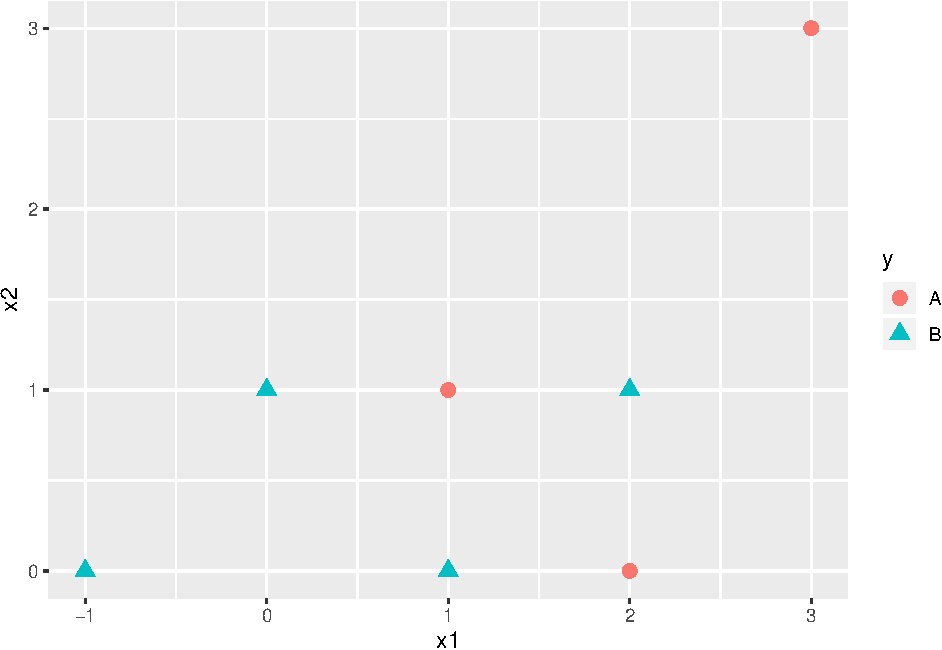
\includegraphics{RecEx4_files/figure-latex/unnamed-chunk-1-1.pdf}

\begin{Shaded}
\begin{Highlighting}[]
\NormalTok{n =}\StringTok{ }\KeywordTok{dim}\NormalTok{(wine)[}\DecValTok{1}\NormalTok{]}
\KeywordTok{set.seed}\NormalTok{(}\DecValTok{4268}\NormalTok{)  }\CommentTok{#to get the same order if you rerun}
\NormalTok{ord =}\StringTok{ }\KeywordTok{sample}\NormalTok{(}\DecValTok{1}\OperatorTok{:}\NormalTok{n)  }\CommentTok{#shuffle, without replacement }
\NormalTok{test =}\StringTok{ }\NormalTok{wine[ord[}\DecValTok{1}\OperatorTok{:}\NormalTok{(n}\OperatorTok{/}\DecValTok{2}\NormalTok{)], ]  }\CommentTok{# first half is test, second train - could have been opposite}
\NormalTok{train =}\StringTok{ }\NormalTok{wine[ord[((n}\OperatorTok{/}\DecValTok{2}\NormalTok{) }\OperatorTok{+}\StringTok{ }\DecValTok{1}\NormalTok{)}\OperatorTok{:}\NormalTok{n], ]}
\end{Highlighting}
\end{Shaded}

In our data the two classes are named \texttt{y} and coded \(Y=0\) and
\(Y=1\), and we name \(x_1\)= \texttt{Alcalinity\_of\_ash}=\texttt{x1}
and \(x_2\)=\texttt{Color\_intensity}=\texttt{x2}.

\subsubsection{a) Logistic regression}\label{a-logistic-regression}

We assume a logistic regression model for observation \(i\),
\(i=1,\ldots,n\): \[
P(Y_i = 1| {\bf X}={\bf x}_i) = p_i = \frac{e^{\beta_0 + \beta_1x_{i1} + \beta_2 x_{i2}}}{ 1+ e^{\beta_0 + \beta_1x_{i1} + \beta_2x_{i2}}}
\]

\begin{itemize}
\tightlist
\item
  Use this expression to show that
  logit\((p_i)=\log(\frac{p_i}{1-p_i})\) is a linear function in \(x_1\)
  and \$x\_2..
\item
  Fit a logistic regression model with model formula
  \texttt{y\textasciitilde{}x1+x2} to the training set.
\item
  Give an interpretation of \(\hat{\beta}_1\) and \(\hat{\beta}_2\).
\item
  We use the rule to classify to class 1 for an observation with
  covariates \({\bf x}\) if \(\hat{\text{Pr}}(Y=1\mid {\bf x})>0.5\).
  Write down the formula for the class boundary between the classes.
  What type of boundary is this?
\item
  Make a plot with the training observations and the class boundary.
  Hint: in \texttt{ggplot} points are added with \texttt{geom\_point}
  and a line with \texttt{geom\_abline(slope=b,\ intercept=a)} where
  \(a\) and \(b\) comes from your class boundary, and title with
  \texttt{ggtitle}.
\item
  Use the \texttt{summary} output to \emph{manually} derive the
  predicted probability \(\hat{\text{Pr}}(Y=1\mid x_1=17, x_2=3)\). What
  is the interpretation of this value?
\item
  Compute predicted probabilites for all observations in the test set.
\item
  Make the confusion table for the test set when using 0.5 as cutoff for
  the probabilities. Calculate the sensitivity and specificity on the
  test set. How would you evaluate the performance of this
  classification?
\end{itemize}

\subsubsection{b) K-nearest neighbor
classifier}\label{b-k-nearest-neighbor-classifier}

To decide the class of an new observation, the KNN classifier uses the
nearest neighbours in the following way, \[
P(Y=1|X=x_0) = \frac{1}{K}\sum_{i\in \mathcal{N_0}}I(y_i=j).
\]

\begin{itemize}
\tightlist
\item
  Explain this expression does, and what the different elements are.
\item
  Use KNN with \(K=3\) to classify the wines in the test set.
\item
  Make the confusion table for the test set when using 0.5 as cutoff.
  Calculate the sensitivity and specificity on the test set. How would
  you evaluate the performance of this classification?
\item
  Repeat with \(K=9\). Which of these two choices of \(K\) would you
  prefer and why? Why don't we just choose \(K\) as high or as low as
  possible?
\end{itemize}

Comment: The following code was not given to the students, but there was
some confusion on the \texttt{KNN3prob} below, so not the code is
included.

\begin{Shaded}
\begin{Highlighting}[]
\NormalTok{KNN3 =}\StringTok{ }\KeywordTok{knn}\NormalTok{(}\DataTypeTok{train =}\NormalTok{ train[, }\DecValTok{-1}\NormalTok{], }\DataTypeTok{test =}\NormalTok{ test[, }\DecValTok{-1}\NormalTok{], }\DataTypeTok{k =} \DecValTok{3}\NormalTok{, }\DataTypeTok{cl =}\NormalTok{ train}\OperatorTok{$}\NormalTok{y, }
    \DataTypeTok{prob =}\NormalTok{ F)}
\NormalTok{t3 =}\StringTok{ }\KeywordTok{table}\NormalTok{(test}\OperatorTok{$}\NormalTok{y, KNN3)}
\NormalTok{t3}
\KeywordTok{apply}\NormalTok{(t3, }\DecValTok{1}\NormalTok{, sum)}
\NormalTok{n =}\StringTok{ }\KeywordTok{length}\NormalTok{(test}\OperatorTok{$}\NormalTok{y)}
\NormalTok{error =}\StringTok{ }\NormalTok{(n }\OperatorTok{-}\StringTok{ }\KeywordTok{sum}\NormalTok{(}\KeywordTok{diag}\NormalTok{(t3)))}\OperatorTok{/}\NormalTok{n}
\NormalTok{error}
\NormalTok{KNN3probwinning =}\StringTok{ }\KeywordTok{attributes}\NormalTok{(}\KeywordTok{knn}\NormalTok{(}\DataTypeTok{train =}\NormalTok{ train[, }\DecValTok{-1}\NormalTok{], }\DataTypeTok{test =}\NormalTok{ test[, }\DecValTok{-1}\NormalTok{], }
    \DataTypeTok{k =} \DecValTok{3}\NormalTok{, }\DataTypeTok{cl =}\NormalTok{ train}\OperatorTok{$}\NormalTok{y, }\DataTypeTok{prob =} \OtherTok{TRUE}\NormalTok{))}\OperatorTok{$}\NormalTok{prob}
\NormalTok{KNN3prob <-}\StringTok{ }\KeywordTok{ifelse}\NormalTok{(KNN3 }\OperatorTok{==}\StringTok{ "0"}\NormalTok{, }\DecValTok{1} \OperatorTok{-}\StringTok{ }\NormalTok{KNN3probwinning, KNN3probwinning)}
\CommentTok{# cbind(KNN3prob,KNN3,KNN3probwinning) to check that this is correct}
\NormalTok{KNN3roc =}\StringTok{ }\KeywordTok{roc}\NormalTok{(}\DataTypeTok{response =}\NormalTok{ test}\OperatorTok{$}\NormalTok{y, }\DataTypeTok{predictor =}\NormalTok{ KNN3prob)}
\KeywordTok{cbind}\NormalTok{(KNN3roc}\OperatorTok{$}\NormalTok{threshold, KNN3roc}\OperatorTok{$}\NormalTok{sens, KNN3roc}\OperatorTok{$}\NormalTok{specificities)}
\end{Highlighting}
\end{Shaded}

\begin{Shaded}
\begin{Highlighting}[]
\NormalTok{KNN9 =}\StringTok{ }\KeywordTok{knn}\NormalTok{(}\DataTypeTok{train =}\NormalTok{ train[, }\DecValTok{-1}\NormalTok{], }\DataTypeTok{test =}\NormalTok{ test[, }\DecValTok{-1}\NormalTok{], }\DataTypeTok{k =} \DecValTok{9}\NormalTok{, }\DataTypeTok{cl =}\NormalTok{ train}\OperatorTok{$}\NormalTok{y, }
    \DataTypeTok{prob =}\NormalTok{ F)}
\NormalTok{t9 =}\StringTok{ }\KeywordTok{table}\NormalTok{(test}\OperatorTok{$}\NormalTok{y, KNN9)}
\NormalTok{t9}
\NormalTok{error =}\StringTok{ }\NormalTok{(n }\OperatorTok{-}\StringTok{ }\KeywordTok{sum}\NormalTok{(}\KeywordTok{diag}\NormalTok{(t9)))}\OperatorTok{/}\NormalTok{n}
\NormalTok{error}
\NormalTok{KNN9probwinning =}\StringTok{ }\KeywordTok{attributes}\NormalTok{(}\KeywordTok{knn}\NormalTok{(}\DataTypeTok{train =}\NormalTok{ train[, }\DecValTok{-1}\NormalTok{], }\DataTypeTok{test =}\NormalTok{ test[, }\DecValTok{-1}\NormalTok{], }
    \DataTypeTok{k =} \DecValTok{9}\NormalTok{, }\DataTypeTok{cl =}\NormalTok{ train}\OperatorTok{$}\NormalTok{y, }\DataTypeTok{prob =} \OtherTok{TRUE}\NormalTok{))}\OperatorTok{$}\NormalTok{prob}
\NormalTok{KNN9prob <-}\StringTok{ }\KeywordTok{ifelse}\NormalTok{(KNN9 }\OperatorTok{==}\StringTok{ "0"}\NormalTok{, }\DecValTok{1} \OperatorTok{-}\StringTok{ }\NormalTok{KNN9probwinning, KNN9probwinning)}
\NormalTok{KNN9roc =}\StringTok{ }\KeywordTok{roc}\NormalTok{(}\DataTypeTok{response =}\NormalTok{ test}\OperatorTok{$}\NormalTok{y, }\DataTypeTok{predictor =}\NormalTok{ KNN9prob)}
\KeywordTok{cbind}\NormalTok{(KNN9roc}\OperatorTok{$}\NormalTok{threshold, KNN9roc}\OperatorTok{$}\NormalTok{sens, KNN9roc}\OperatorTok{$}\NormalTok{specificities)}
\KeywordTok{table}\NormalTok{(KNN3, KNN9)}
\end{Highlighting}
\end{Shaded}

\subsubsection{c) LDA (\& QDA)}\label{c-lda-qda}

In linear discriminant analysis, with \(K\) classes, we assign a class
to a new observation based on the posterior probability

\[P(Y=k | {\bf X}={\bf x}) = \frac{\pi_k f_k({\bf x})}{\sum_{l=1}^K \pi_l f_l({\bf x})},\]
where
\[f_k({\bf x}) = \frac{1}{(2 \pi)^{p/2}|\boldsymbol{\Sigma}|^{1/2}}e^{-\frac{1}{2}({\bf x}-\boldsymbol{\mu_k})^T \boldsymbol{\Sigma}^{-1}({\bf x}-\boldsymbol{\mu_k})}.\]

\begin{itemize}
\tightlist
\item
  Explain what is \(\pi_k\), \(\boldsymbol{\mu}_k\),
  \(\boldsymbol{\Sigma}\) and \(f_k(x)\) in our \texttt{wine} problem.
\item
  How can we estimate \(\pi_k\), \(\boldsymbol{\mu}_k\) and
  \(\boldsymbol{\Sigma}\)? Compute estimates for these quantities based
  on the training set.
\end{itemize}

In a two class problem (\(K=2\)) the decision boundary for LDA between
class 0 and class 1 is where \(x\) satisfies \[
P(Y=0 | {\bf X}={\bf x}) = P(Y=1 | {\bf X}={\bf x}).
\]

\begin{itemize}
\tightlist
\item
  Show that we can express this as

  \begin{align}
  \delta_0({\bf x}) &= \delta_1({\bf x}),
  \end{align}

  where

  \begin{align}
  \delta_k({\bf x}) &= {\bf x}^T \boldsymbol{\Sigma}^{-1}\boldsymbol{\mu}_k - \frac{1}{2}\boldsymbol{\mu}_k^T \boldsymbol{\Sigma}^{-1}\boldsymbol{\mu}_k + \log \pi_k; \quad k\in\{0,1\}.
  \end{align}
\item
  Perform LDA on the training data (using R).
\item
  We use the rule to classify to class 1 for an observation with
  covariates \({\bf x}\) if \(\hat{P}(Y=1\mid {\bf x})>0.5\). Write down
  the formula for the class boundary between the classes.
\item
  Make a plot with the training observations and the class boundary. Add
  the test observations to the plot (different markings). Hint: in
  \texttt{ggplot} points are added with \texttt{geom\_points} and a line
  with \texttt{geom\_abline(slope=b,\ intercept=a)} where \(a\) and
  \(b\) comes from your class boundary.
\item
  Make the confusion table for the test set when using 0.5 as cut-off.
  Calculate the sensitivity and specificity on the test set. How would
  you evaluate the performance of this classification?
\item
  If you where to perform QDA instead of LDA, what would be the most
  important difference between the QDA and LDA philosophy?
\end{itemize}

\subsubsection{d) Compare classifiers}\label{d-compare-classifiers}

\begin{itemize}
\tightlist
\item
  Compare your results from the different classification methods
  (logistic regression, your preferred KNN, LDA) based on the 0.5
  cut-off on posterior probability classification rule. Which method
  would you prefer?
\item
  Explain what an ROC curve is and why that is useful. Would your
  preference (to which method is the best for our data) change if a
  different cut-off was chosen? Answer this by producing ROC-curves for
  the three methods on the test set. Also calculate AUC. Hint: use
  function \texttt{res=roc(response=test\$y,predictor)} in
  \texttt{library(pROC)} where the predictor is a vector with your
  predicted posterior probabilites for the test set, and then
  \texttt{plot(res)} and \texttt{auc(res)}.
\end{itemize}

\section{Old exam problems (not sure to keep them here - ev. better to
give full exam at a later point in the
course?)}\label{old-exam-problems-not-sure-to-keep-them-here---ev.-better-to-give-full-exam-at-a-later-point-in-the-course}

\subsection{Problem 9 (from exam 2018)}\label{problem-9-from-exam-2018}

In this problem you may use that the probability density function for a
\(p\)-dimensional multivariate normal random variable \({\bf X}\) with
mean \({\boldsymbol \mu}\) and variance-covariance matrix
\({\boldsymbol \Sigma}\) is given as:
\[f({\bf x}) = \frac{1}{(2 \pi)^{p/2}|\boldsymbol{\Sigma}|^{1/2}}\exp({-\frac{1}{2}({\bf x}-\boldsymbol\mu)^T \boldsymbol{\Sigma}^{-1}({\bf x}-\boldsymbol\mu)})\]
We will not discuss how to estimate the mean and variance-covariance
matrix here, so you may assume that they are known.

\textbf{Q10:} Write down the mathematical model assumptions for a linear
discriminant analysis with two classes (coded as 0 and 1) and \(p\)
explanatory variables and explain what the different ingredients are.

\textbf{Q11:} Explain how you derive the mathematical formula for the
posterior probability for class 1.

\textbf{Q12:} Derive the mathematical formula for the class boundary
between the two classes, given that the classification rule is to
classify to the class with the highest posterior probability.

\textbf{Q13:} Is this boundary linear or non-linear in the space of the
explanatory variables?

\subsection{Problem 10 (from exam
2018)}\label{problem-10-from-exam-2018}

We will look at data on diabetes (\texttt{diabetes} is \texttt{0} if not
present and \texttt{1} if present) from a population of women of Pima
Indian heritage in the US, available in the R \texttt{MASS} package. The
following covariates were collected for each woman:

\begin{itemize}
\tightlist
\item
  \texttt{npreg}: number of pregnancies
\item
  \texttt{glu}: plasma glucose concentration in an oral glucose
  tolerance test
\item
  \texttt{bp}: diastolic blood pressure (mmHg)
\item
  \texttt{skin}: triceps skin fold thickness (mm)
\item
  \texttt{bmi}: body mass index (weight in kg/(height in m)\(^2\))
\item
  \texttt{ped}: diabetes pedigree function.
\item
  \texttt{age}: age in years
\end{itemize}

We will use a training set (called \texttt{train}) with 200 observations
(132 non-diabetes and 68 diabetes cases) and a test set (called
\texttt{test}) with 332 observations (223 non-diabetes and 109 diabetes
cases). Our aim is to make a classification rule for diabetes (or not)
based on the available data.

Below you find R-code and results from fitting a logistic regression to
the \texttt{train} data set.

\textbf{Q14:} Write down the statistical model for the logistic
regression.

\textbf{Q15:} Explain what is the estimated effect of the \texttt{ped}
covariate on getting diabetes.

\textbf{Q16:} Would you predict that a person with the following
characteristics has diabetes?

Person: \texttt{npreg}=2, \texttt{glu}=145, \texttt{bp}=85,
\texttt{skin}=35, \texttt{bmi}=37, \texttt{ped}=0.7, \texttt{age}=40.

\textbf{Q17:} Draw a feedforward neural network with the same
architecture as the logistic regression and specify which activation
function(s) is/are used. Label nodes and connections with the same
notation as for the mathematical model for the logistic regression.

The \texttt{test} data set was used to evaluate the performance of the
logistic regression. A receiver--operator curve (ROC) was constructed
and is the solid curve in the figure below (the dotted and dashed curves
will be studie in Q24).

\textbf{Q18:} Explain briefly how a ROC curve is constructed. Your
explanation should include the words cut-off, confusion matrix,
sensitivity, specificity.

Look at the confusion matrix (probability cut-off 0.5) reported for the
test set in the bottom part of the print-out in the figure below.

\textbf{Q19:} Which point on the ROC curve does this cut-off correspond
to?

\begin{verbatim}
# logistic regression
> fitlogist=glm(diabetes~npreg+glu+bp+skin+bmi+ped+age,data=train,
family=binomial(link="logit"))
> summary(fitlogist)
Call:
glm(formula = diabetes ~ npreg + glu + bp + skin + bmi + ped + 
    age, family = binomial(link = "logit"), data = train)
Coefficients:
             Estimate Std. Error z value Pr(>|z|)    
(Intercept) -9.773062   1.770386  -5.520 3.38e-08 ***
npreg        0.103183   0.064694   1.595  0.11073    
glu          0.032117   0.006787   4.732 2.22e-06 ***
bp          -0.004768   0.018541  -0.257  0.79707    
skin        -0.001917   0.022500  -0.085  0.93211    
bmi          0.083624   0.042827   1.953  0.05087 .  
ped          1.820410   0.665514   2.735  0.00623 ** 
age          0.041184   0.022091   1.864  0.06228 .  
---
Signif. codes:  0 '***' 0.001 '**' 0.01 '*' 0.05 '.' 0.1 ' ' 1
(Dispersion parameter for binomial family taken to be 1)
    Null deviance: 256.41  on 199  degrees of freedom
Residual deviance: 178.39  on 192  degrees of freedom
AIC: 194.39
Number of Fisher Scoring iterations: 5

> predlogist=predict(fitlogist,newdata=test,type="response")
> testclasslogist=ifelse(predlogist > 0.5, 1, 0)
> table(test$diabetes, testclasslogist)
   testclasslogist
      0   1
  0 200  23
  1  43  66
>  # note: 223 true non-diabetes and 109 true diabetes cases
> library(pROC)
> roclogist=roc(test$diabetes,predlogist)
> auc(roclogist)
Area under the curve: 0.8659
> plot(roclogist, lty="solid")
\end{verbatim}

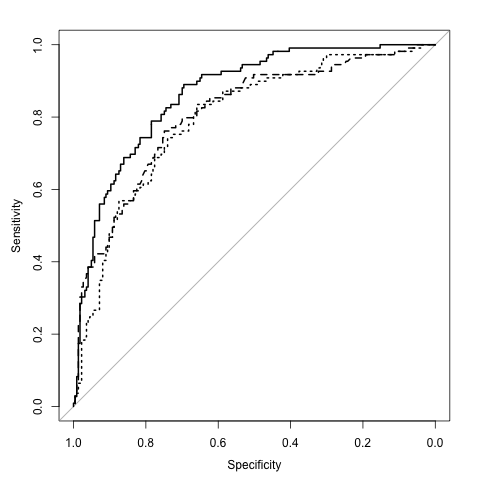
\includegraphics[width=300pt]{ROC}

ROC-curves for logistic (solid), bagged trees (dashed) and quadratic
discriminant analysis (dotted) for the diabetes test data set.


\end{document}
